\documentclass[a4paper,landscape]{article}
\usepackage[utf8]{inputenc}
\usepackage{graphicx}
\usepackage{float}
\usepackage{geometry}
\geometry{margin=1in}
\usepackage{caption}
\usepackage{hyperref}
\usepackage{xcolor}

\title{Data Visualization Portfolio}
\author{Alan Copa}
\date{Data Analytics for Finance I \& II, 2024-2025}

\begin{document}
\maketitle
\begin{figure}[H]
    \centering
    \includegraphics[width=0.31\textwidth]{Visualizations/DALL·E 2025-01-13.pdf}
\end{figure}

\tableofcontents


\section{Introduction}
This portfolio presents a collection of data visualizations created as part of the course Data Analytics for Finance I \& II requirements for the 2024-2025 academic year.

\section{Visualization Tasks}

\subsection{Task 1: Bad/Manipulative Visualization}
\begin{figure}[H]
    \centering
    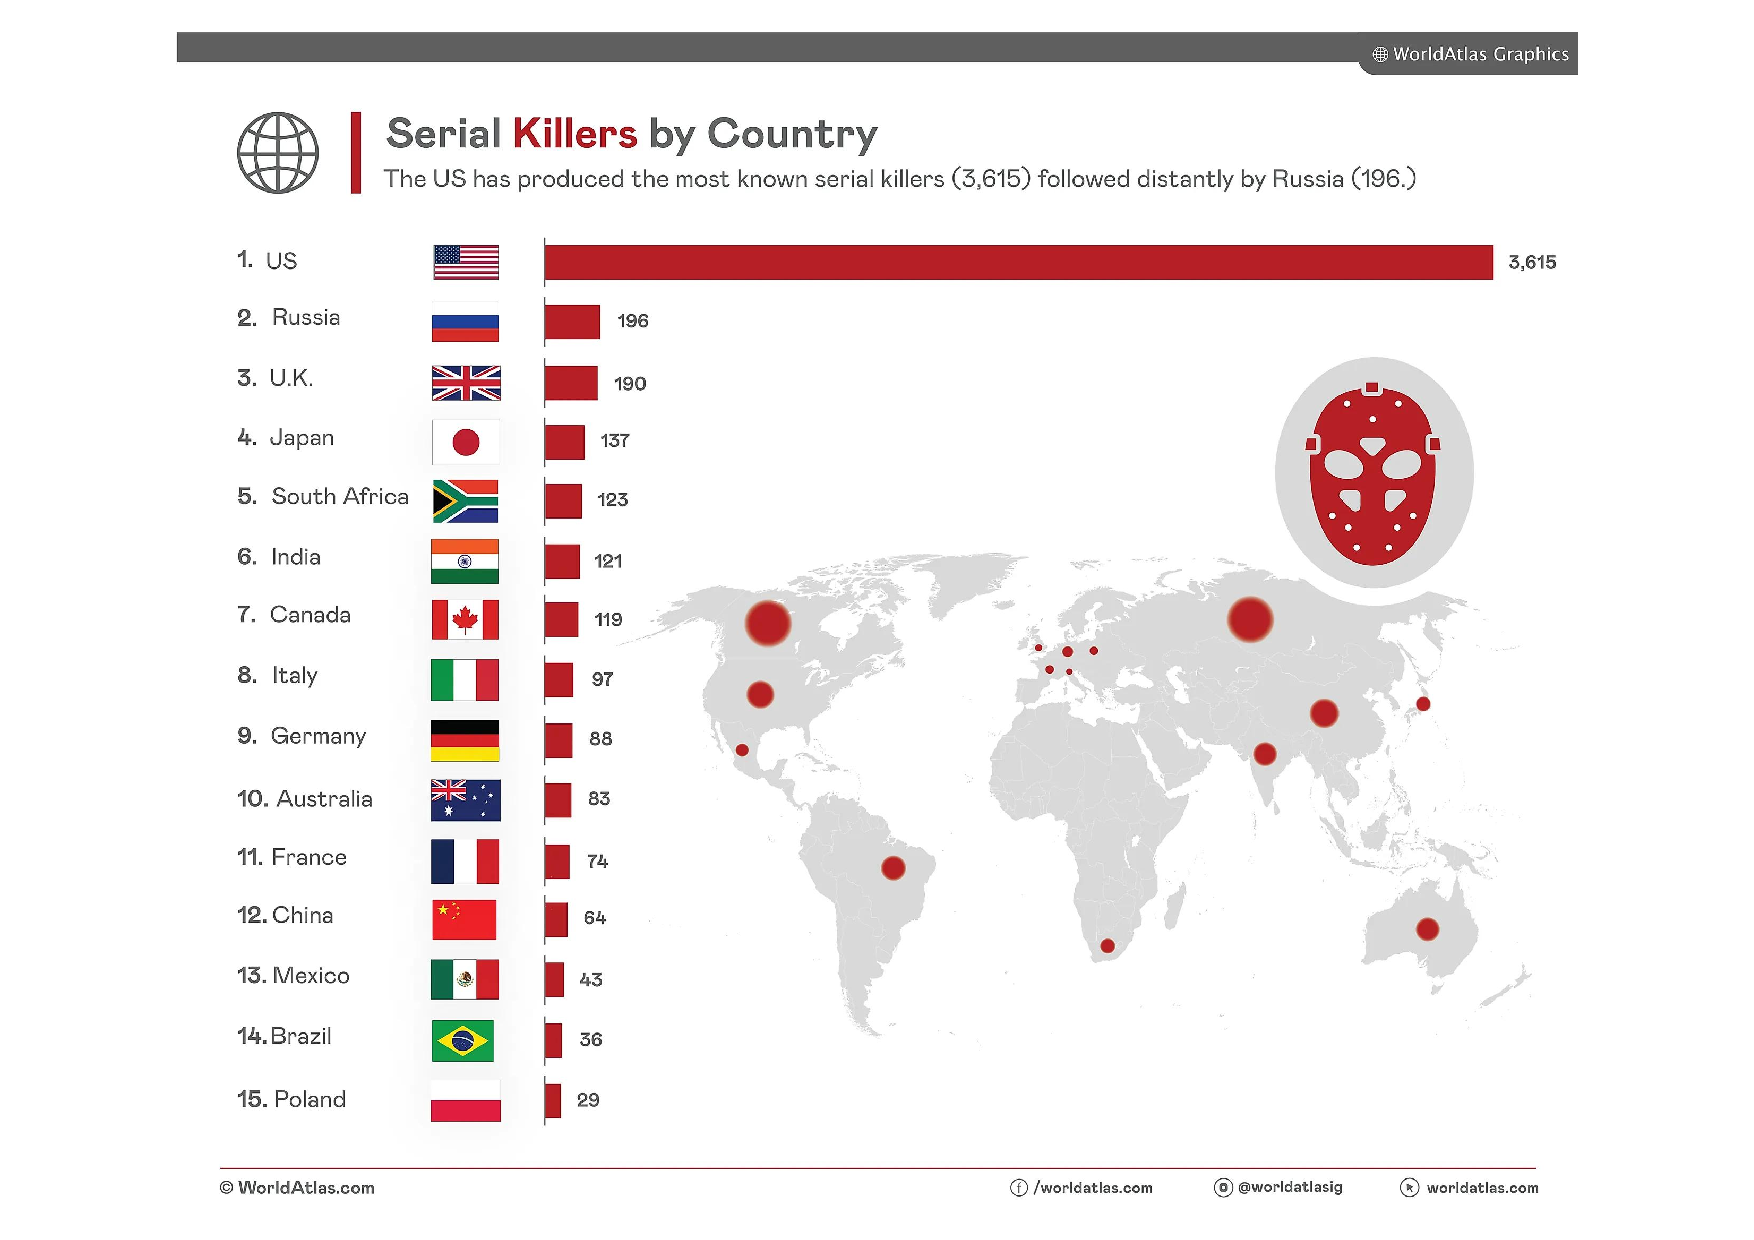
\includegraphics[width=0.8\textwidth]{bad-data.pdf} % Replace with your file name
    \caption{Bad Visualization \cite{worldatlas2025serialkillers}}
    \label{fig:bad}
\end{figure}

\subsubsection{Critique}
This data visualization is misleading because the values in the horizontal bar chart are presented as the absolute number of serial killers per country. The proportion relative to the population of each country is not considered, resulting in an overwhelming scale for the US, which overshadows the other values. The addition of the map without a proper legend adds confusion, as the red circles are not proportional to the data shown. This suggests an alternative perspective but fails to clarify it. Consequently, the presence of two visualization styles is redundant, as it does not provide new insights but instead increases cognitive load. Finally, the inclusion of a mask illustration is purely decorative and does not contribute any functional value to the visualization.

\subsection{Task 2: Improved Bad Visualization}
\begin{figure}[H]
    \centering
    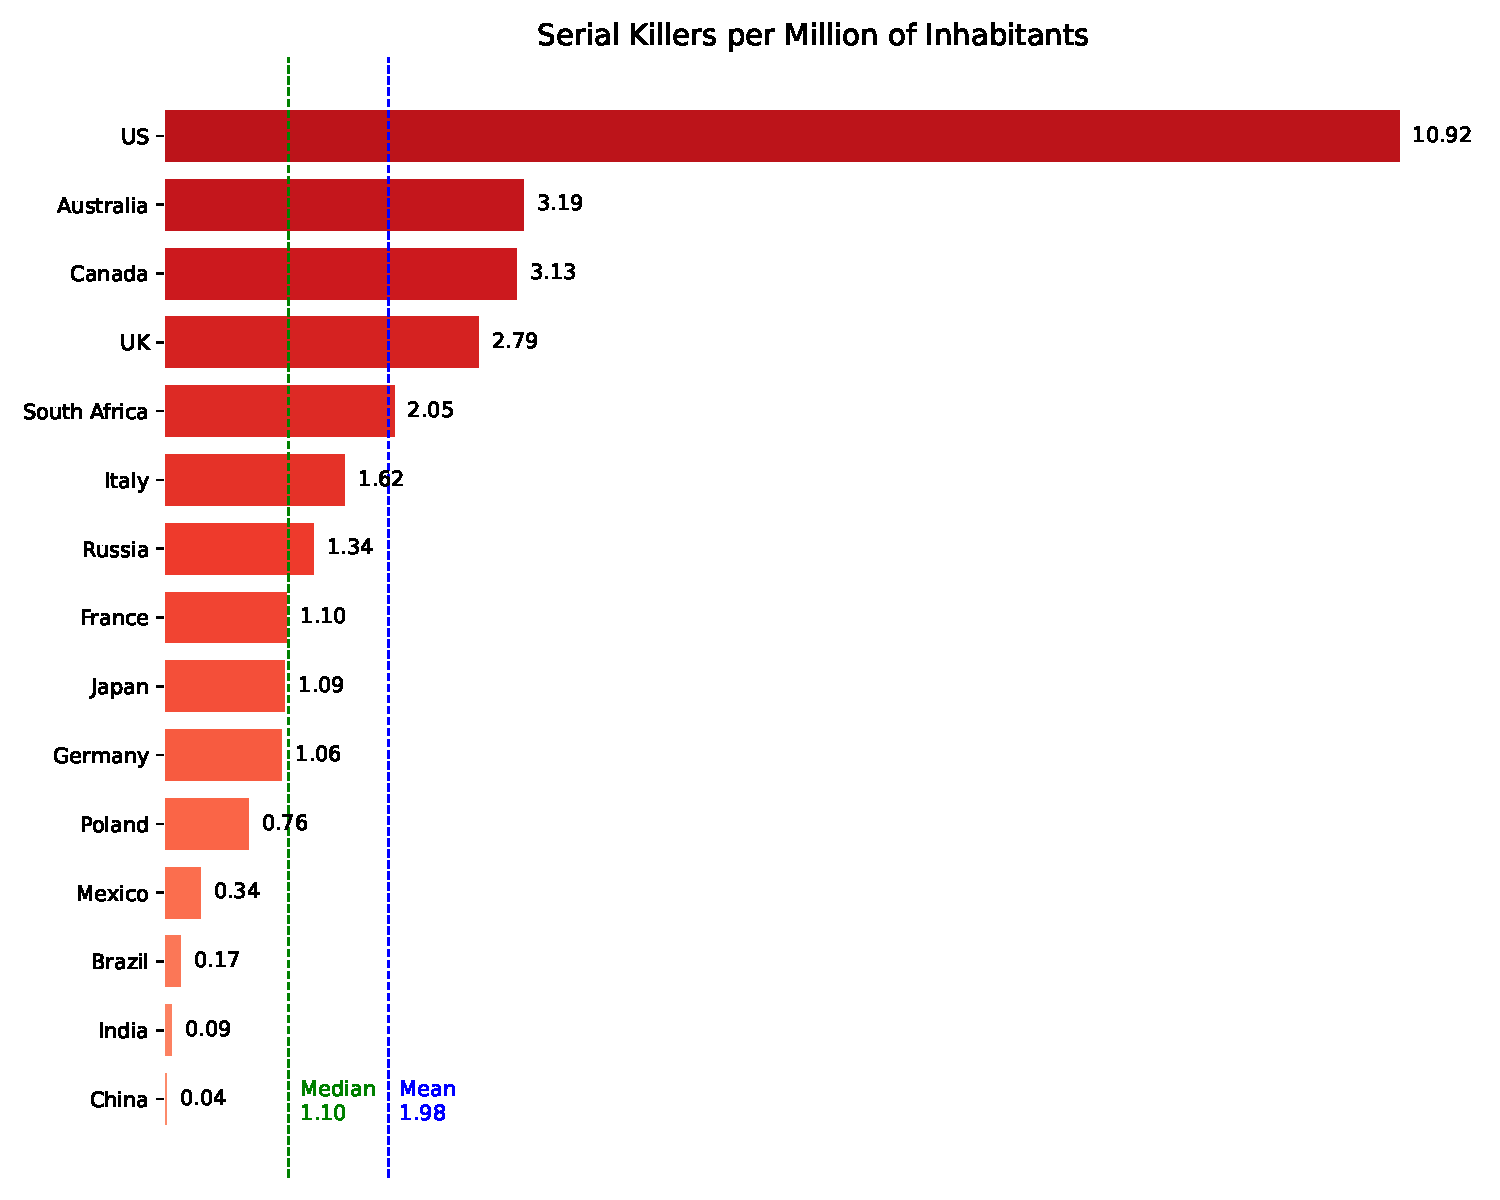
\includegraphics[width=0.8\textwidth]{serial_killers_per_million.pdf} % Replace with your file name
    \caption{Improved version of the bad visualization, Source\cite{worldatlas2025serialkillers}}
    \label{fig:improved}
\end{figure}

\subsection{Task 3: Good Visualization Critique}
\begin{figure}[H]
    \centering
    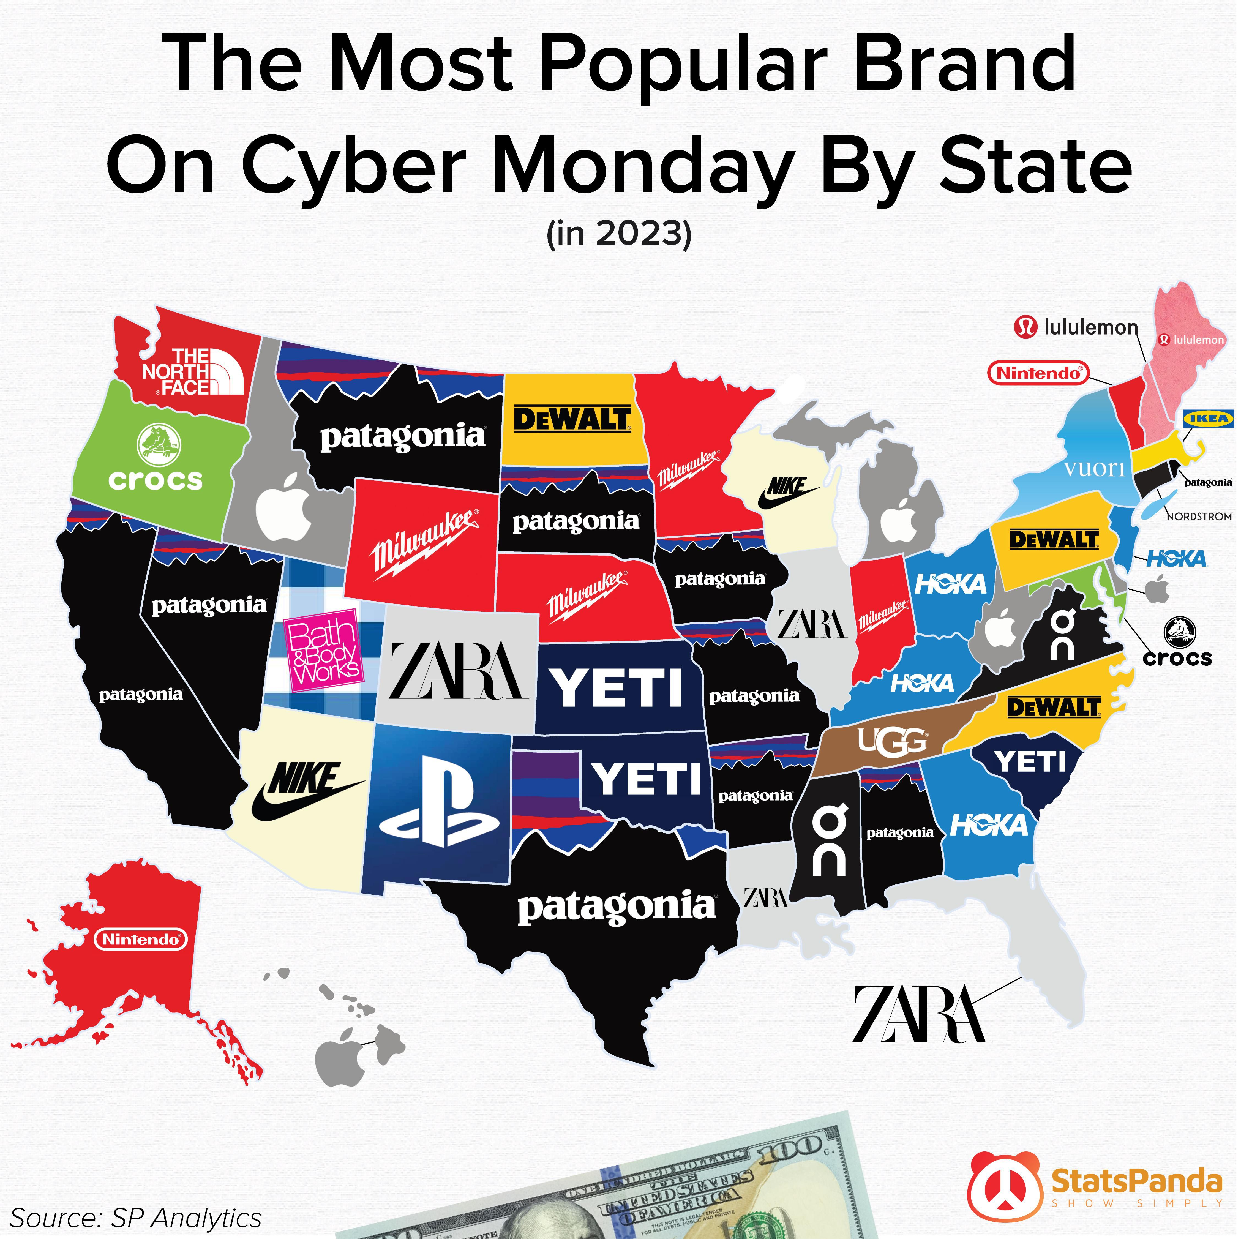
\includegraphics[width=0.6\textwidth]{Visualizations/good-data.pdf} % Replace with your file name
    \caption{Good Visualization, Source \cite{reddit2025cyberbrands}}
    \label{fig:popBrand}
\end{figure}
\subsubsection{Critique}
The visualization is clear at first look. The observer does not need to carefully read any axis or legend. Thanks to the prominent title, the theme of the visualization is easily recognizable, and the recognizable logos make its interpretability straightforward. The colors utilized are associated with the brands and differ from one another, emphasizing the state shapes and enhancing engagement. This visualization is perfect for the general public, as it is simple and colorful. More importantly, it avoids complex data such as numbers or units of measurement, making the message elementary and direct. If it were accompanied by another visualization with more specific data or had an interactive element allowing users to overlay and access additional data, the visualization could be perfect.

\subsection{Task 4: Climate Change Visualization for Social Media}
\subsubsection{The Ozone Layer: Evidence of Global Environmental Action}

\begin{figure}[H]
    \centering
    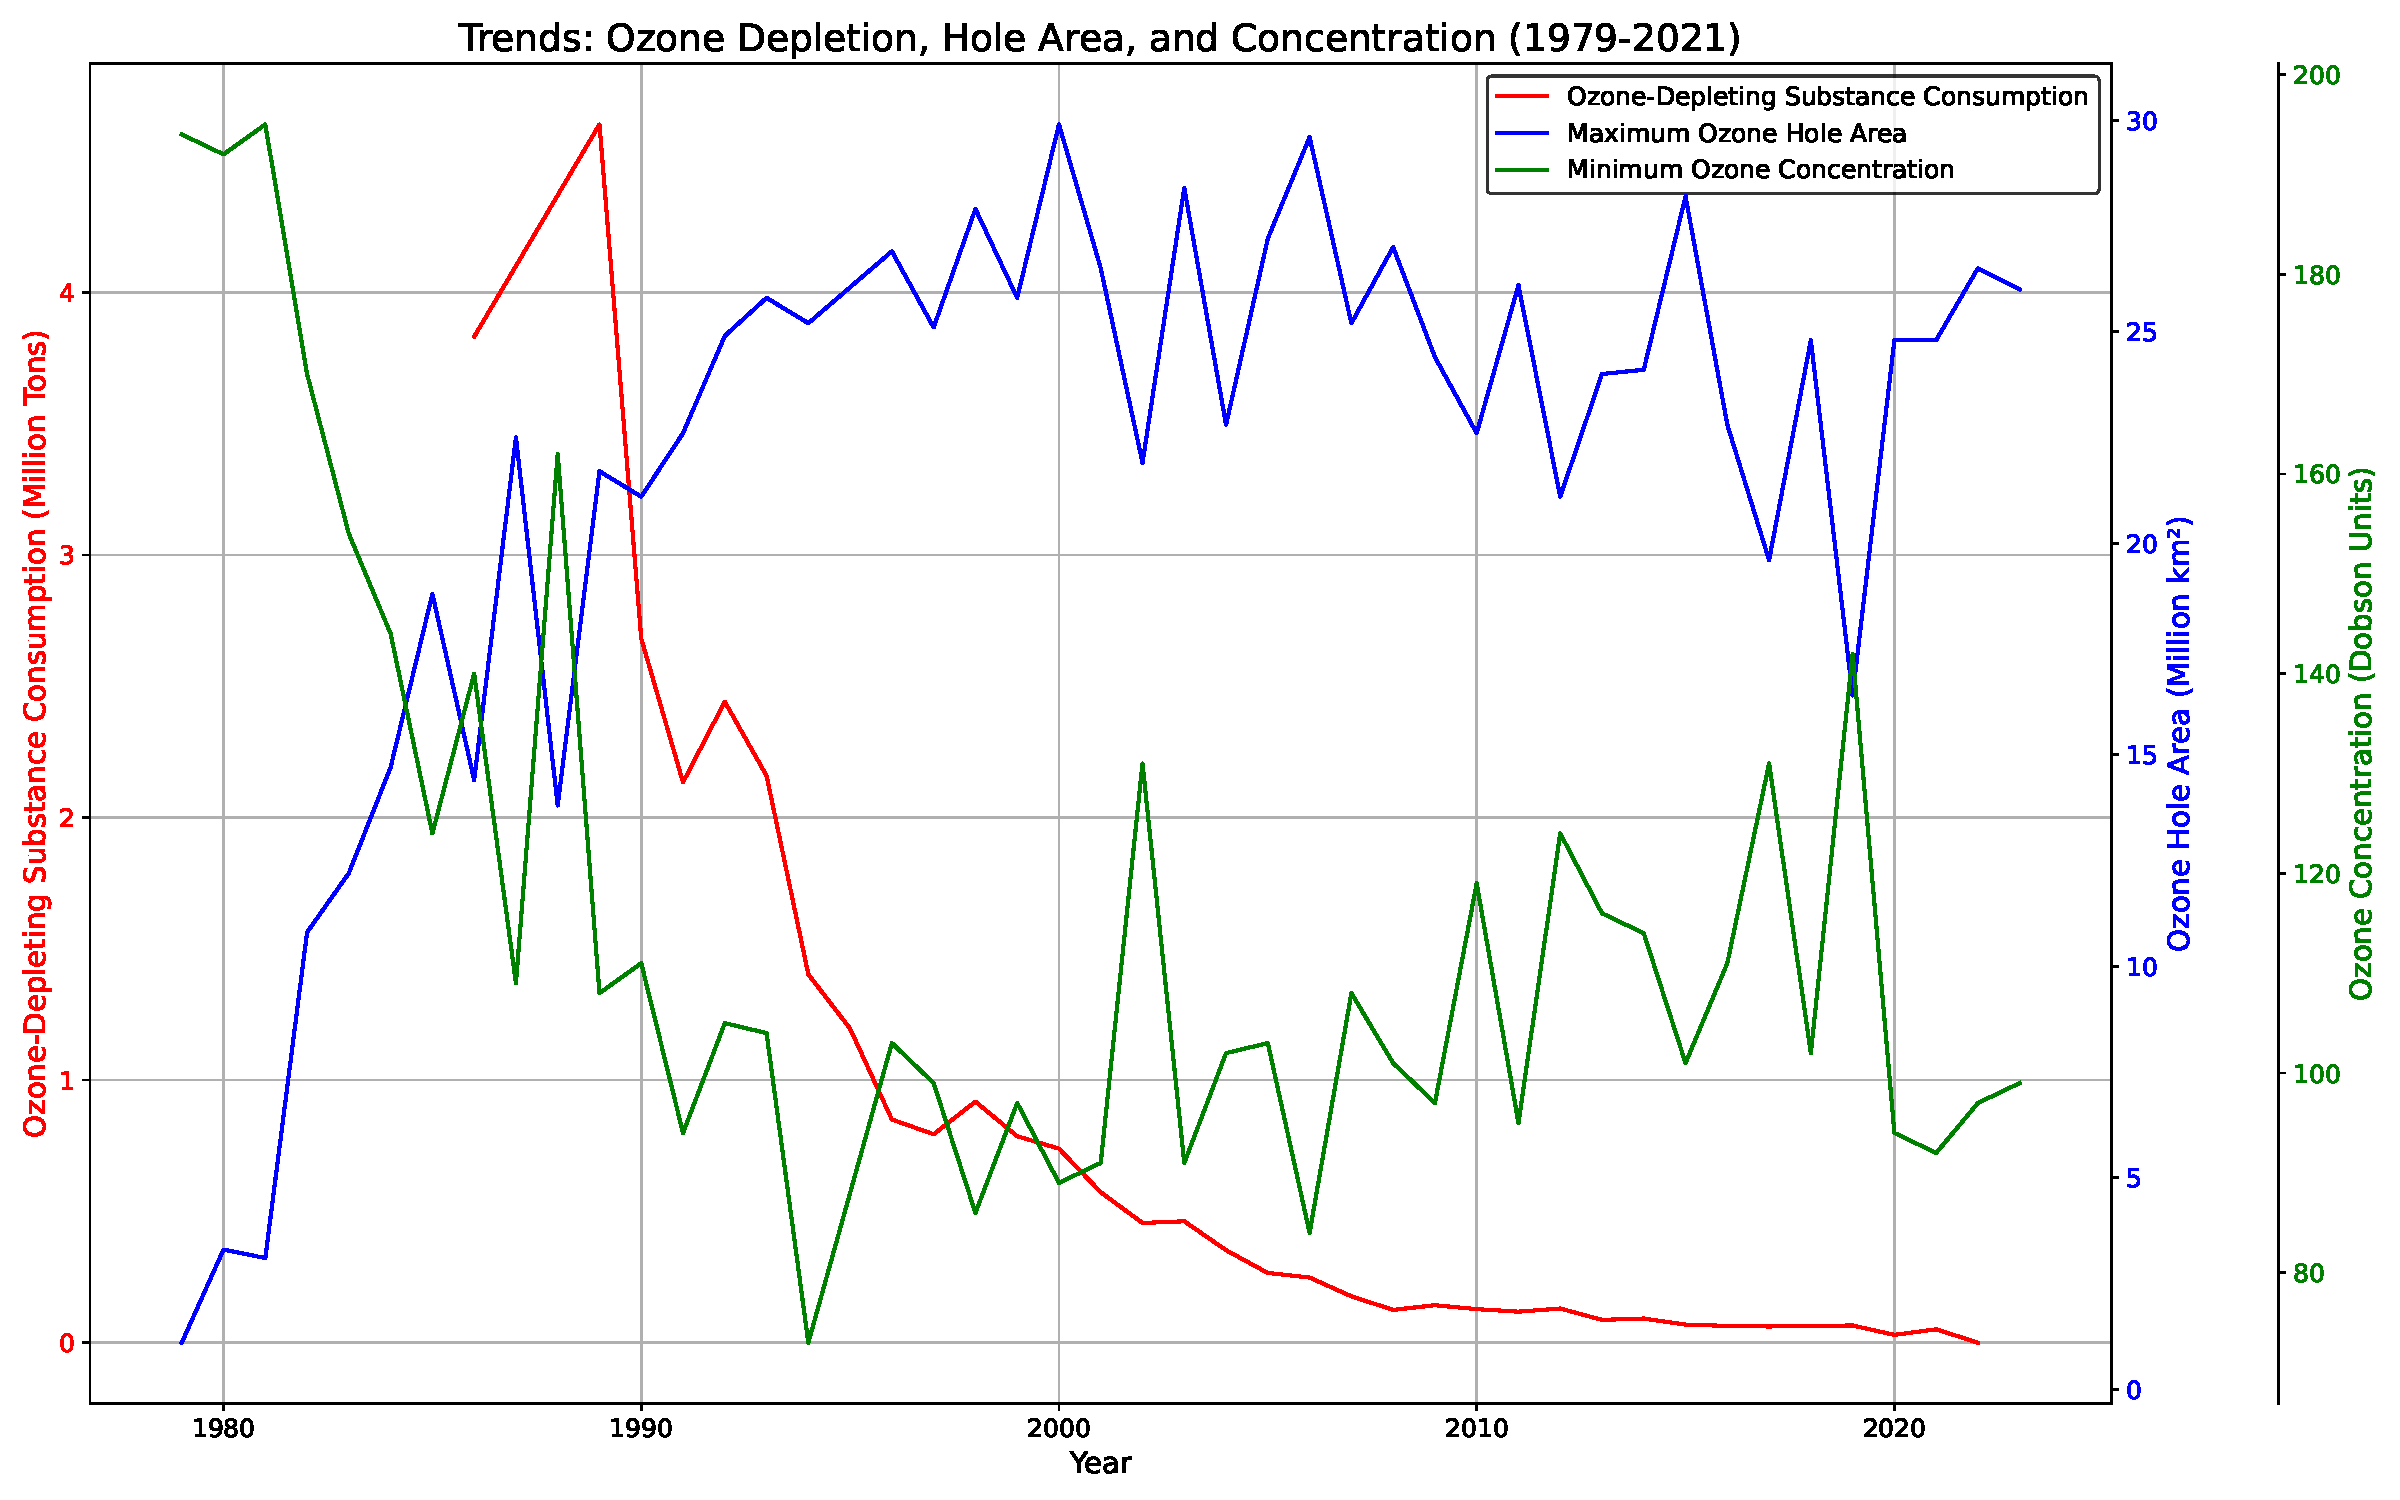
\includegraphics[width=0.8\textwidth]{ozone_data_visualization_t4.pdf} % Replace with your file name
    \caption{Climate change visualization for social media, Source \cite{nasa2024ozone}}
    \label{fig:climate}
\end{figure}

\subsubsection{LinkedIn Post: Healing the Ozone – A Lesson for Climate Change}

\textbf{What is the ozone layer, and why does it matter?}  \\
The Earth's protective shield, the ozone layer, blocks the Sun's damaging ultraviolet (UV) rays. Without it, there would be serious repercussions for life on Earth, such as a rise in skin cancer and ecological disruption. \\ \\ 
\textbf{A brief story of the ozone crisis:} \\
In the 20th century, a massive hole in the ozone layer appeared, especially over Antarctica. This was caused by harmful chemicals like chlorofluorocarbons (CFCs). In response, the 1987 \textit{Montreal Protocol} brought countries together to phase out these chemicals.
As shown in the graph, after the treaty, emissions of ozone-depleting substances began to decline. At the same time, ozone levels stopped decreasing, and the ozone hole stabilized.
The \textit{Montreal Protocol} remains one of the greatest environmental successes, proving that global action can solve even the biggest challenges. \\ \\
\textbf{Climate change lessons:} \\
The data in this visualization tells a crucial story. While the ozone layer’s destruction has slowed, its healing is \textbf{agonizingly slow}—decades after our intervention, the ozone hole persists. This serves as a clear reminder:  
\begin{itemize}
    \item As a species, we hold the power to both harm and heal the environment.
    \item Combating climate crises like global warming requires \textbf{unprecedented global collaboration}.
    \item The healing process of nature is gradual and perhaps irreparable. Time is of the essence.
\end{itemize}
Before the window of opportunity closes, let's take bold action to address climate change, just as we did with ozone depletion. We can guarantee a more sustainable and healthy earth if we work together!


\subsection{Task 5: Black-and-White Visualization}
\textbf{Description:} A visualization using only black and white, with no shades of gray.

\begin{figure}[H]
    \centering
    % \includegraphics[width=0.8\textwidth]{bw_viz.png} % Replace with your file name
    \caption{Black-and-white visualization.}
    \label{fig:bw}
\end{figure}

\textbf{Disclosure:} This graph was generated using OpenAI tools to assist with data analysis and visualization. All data inputs and final outputs were reviewed and validated for accuracy.

\subsection{Task 6: Visualization with Color as a Key Aesthetic}
\textbf{Description:} A visualization that emphasizes the use of color to convey information.

\begin{figure}[H]
    \centering
    % \includegraphics[width=0.8\textwidth]{color_viz.png} % Replace with your file name
    \caption{Visualization utilizing color as a key aesthetic.}
    \label{fig:color}
\end{figure}

\subsection{Task 7:}


\subsection{Task 8: Data Map}
\subsubsection{Average American Expenditure 2023}
\begin{figure}[H]
    \centering
    \caption{Source \cite{bls2025expenditure}}
    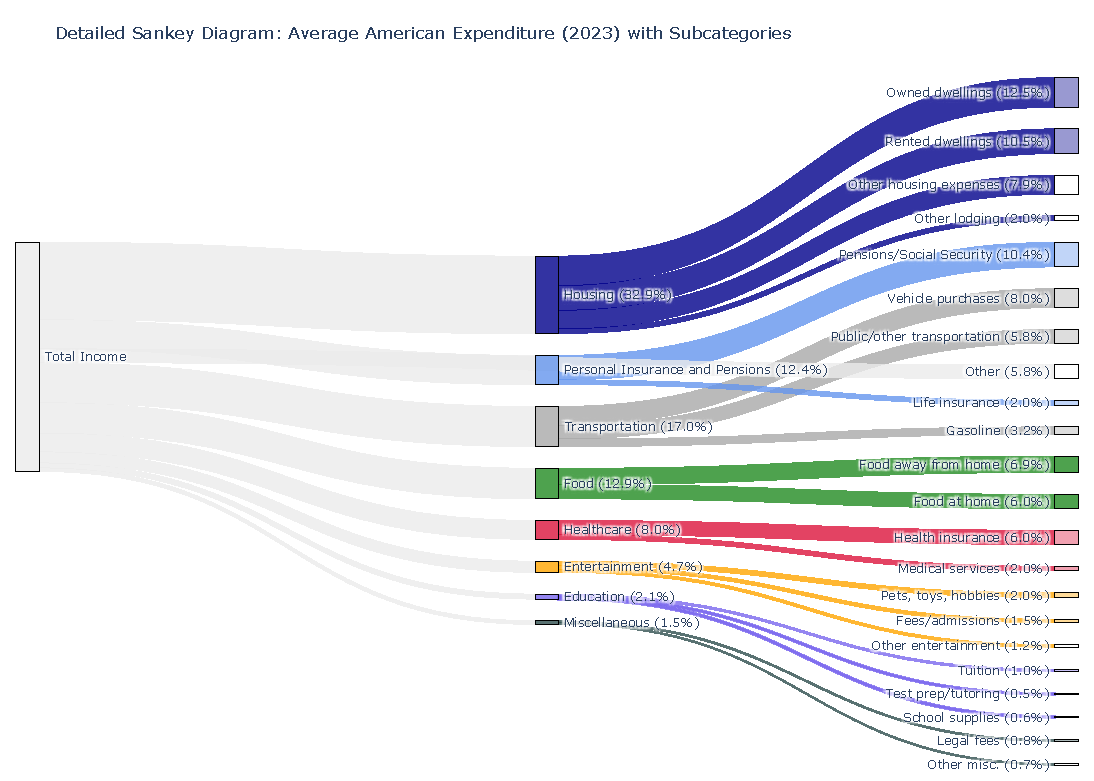
\includegraphics[width=0.9\textwidth]{sankey_diagram.pdf} % Replace with your file name
    \label{fig:americanExp}
\end{figure}

\subsection{Task 11: Data Map}
\subsubsection{inflation rate}

\begin{figure}[H]
    \centering
    % \includegraphics[width=0.8\textwidth]{?.pdf} % Replace with your file name
    \caption{}
    \label{fig:inflation}
\end{figure}

\subsection{Task 14: More Visualizations}
\subsubsection{Measures history of Gravitational Constant G}

\begin{figure}[H]
    \centering
    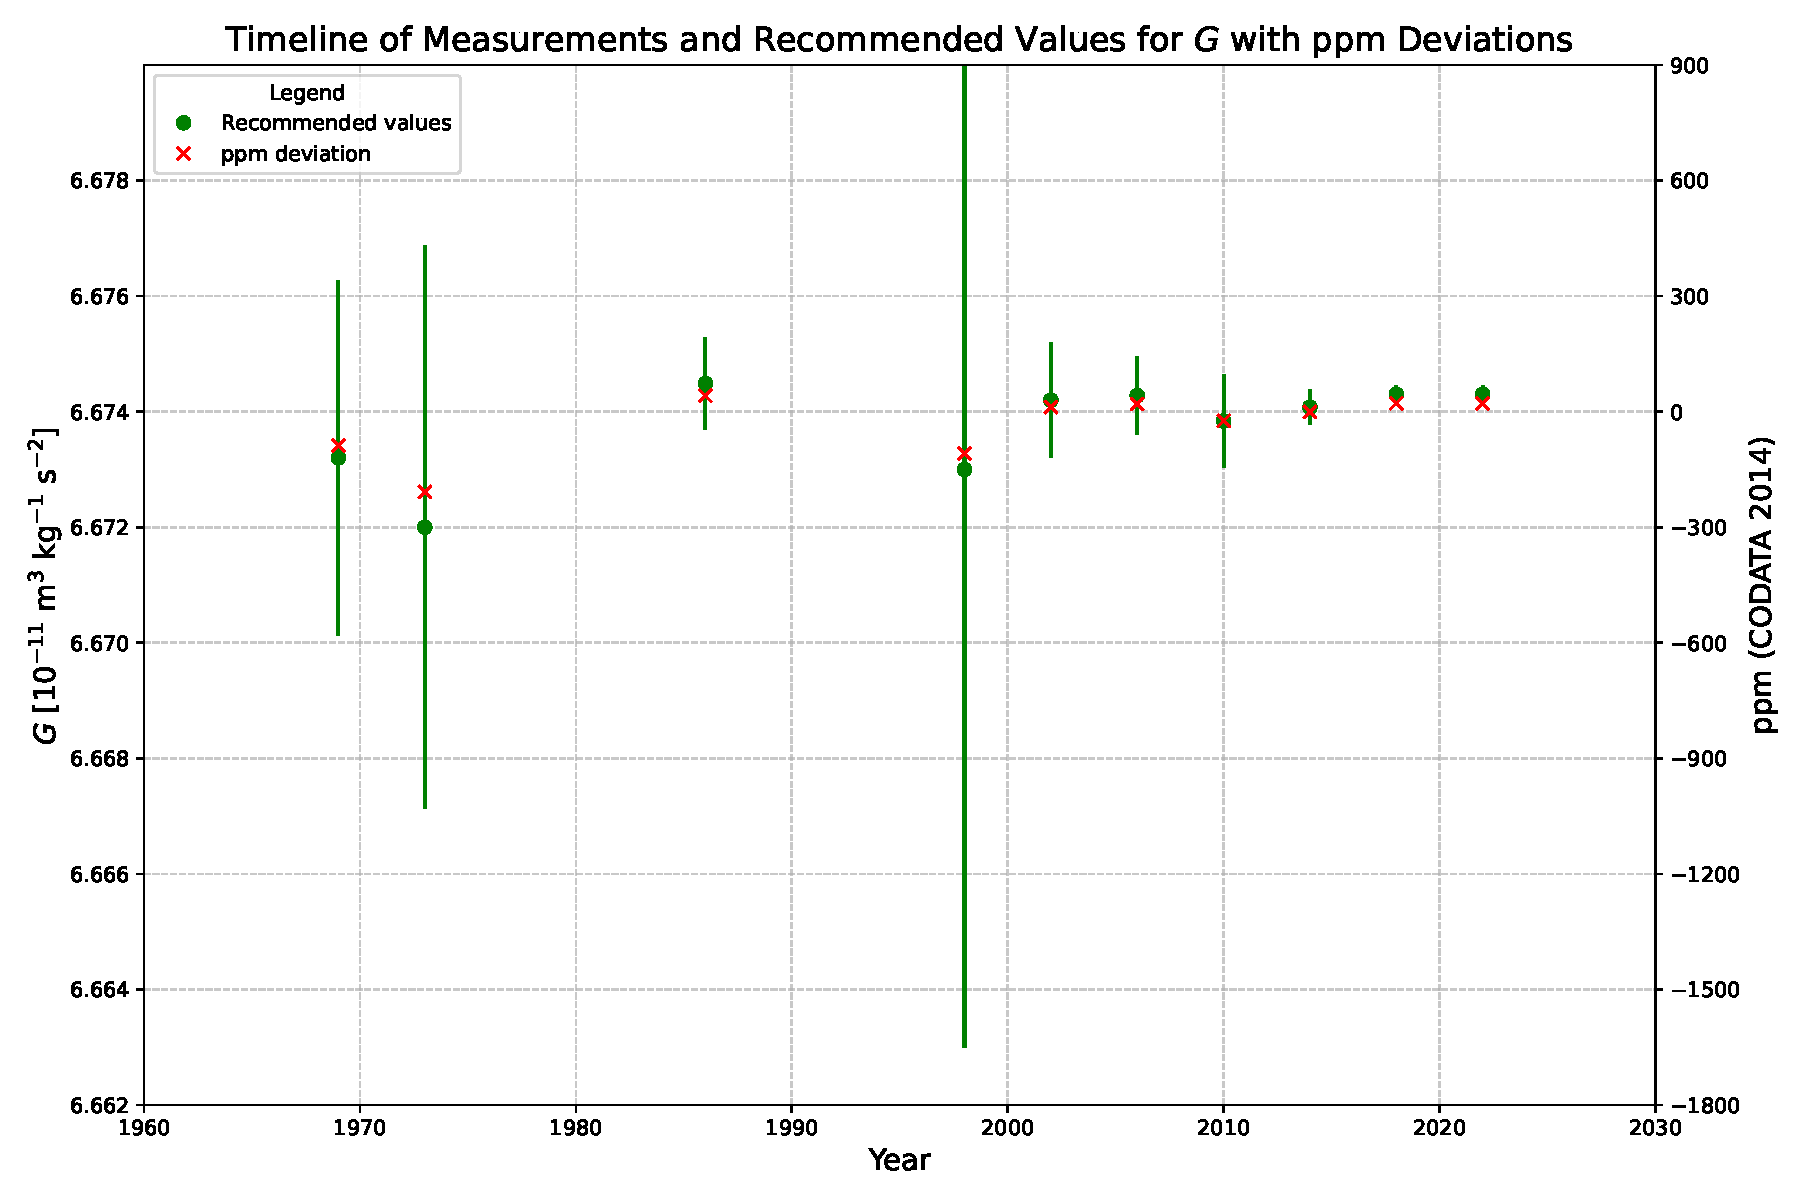
\includegraphics[width=0.8\textwidth]{gravitational_constant.pdf} % Replace with your file name
    \caption{Source \cite{wikipedia2025gconst}}
    \label{fig:G}
\end{figure}


\textbf{Disclosure:} This graph was generated using OpenAI tools to assist with data analysis and visualization. All data inputs and final outputs were reviewed and validated for accuracy.

\section{Bibliography}
\bibliographystyle{abbrv}
\bibliography{references}
\subsection{Data Sources}

\subsection{Software and Tools Used:}
% [List all tools, packages, and software used.]
Python Packages
\begin{itemize}
    \item matplotlib, numpy, pandas, plotly, dash, os, subprocess
\end{itemize}
Software
\begin{itemize}
    \item Visual Studio Code, GPT-4o, My GPTs
\end{itemize}

\subsection{Generative AI Disclosure:}
\begin{itemize}
    \item Task 4: Used ChatGPT Pro to generate Python script for bar chart.
\end{itemize}

\section{Appendix}
\textbf{Screenshots of AI Conversations:}
[Insert screenshots or documentation here.]

\end{document}
